% fig08_equinoctial_frame.tex
% Standalone TikZ: Equinoctial reference frame (f-hat, g-hat, w-hat)
% and definitions of p1, p2, q1, q2
\documentclass[tikz,border=5pt]{standalone}
\usepackage{amsmath,amssymb}
\usetikzlibrary{arrows.meta,calc,decorations.pathreplacing,decorations.markings,
                positioning,3d,angles,quotes}

\definecolor{accent}{RGB}{0, 100, 170}
\definecolor{highlight}{RGB}{200, 60, 30}
\definecolor{darkgreen}{RGB}{0, 120, 60}
\definecolor{earthblue}{RGB}{40,80,150}
\definecolor{orbitgray}{RGB}{100,100,100}

\begin{document}
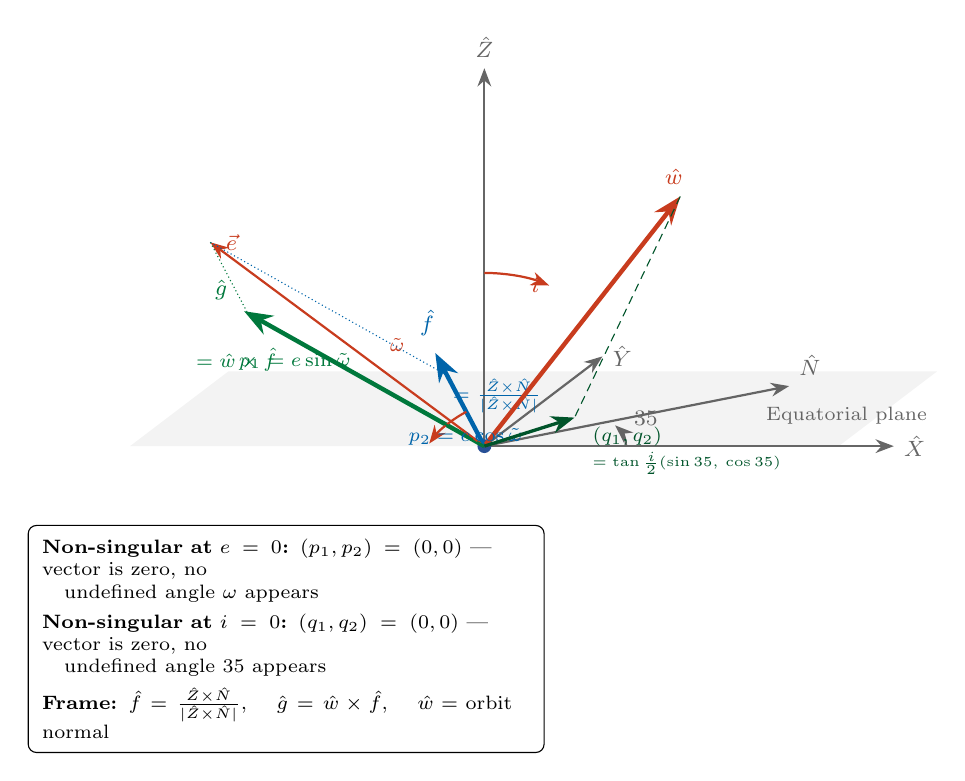
\begin{tikzpicture}[
    >=Stealth,
    font=\footnotesize,
    scale=1.0,
  ]

  %% ── Projection transforms ──
  % Equatorial plane: foreshortened Y
  \pgfmathsetmacro{\eqYx}{0.50}
  \pgfmathsetmacro{\eqYy}{0.38}

  %% ── Equatorial plane fill ──
  \begin{scope}[opacity=0.08]
    \fill[orbitgray]
      (-4.5, 0) -- ({4.5}, 0) --
      ({4.5 + 2.5*\eqYx}, {2.5*\eqYy}) -- ({-4.5 + 2.5*\eqYx}, {2.5*\eqYy})
      -- cycle;
  \end{scope}
  \node[orbitgray, anchor=south] at ({4.0 + 1.2*\eqYx}, {1.2*\eqYy - 0.3})
    {\scriptsize Equatorial plane};

  %% ── Inertial axes ──
  \draw[->, thick, black!60] (0,0) -- (5.2, 0)
    node[right] {$\hat{X}$};
  \draw[->, thick, black!60] (0,0) -- ({3.0*\eqYx}, {3.0*\eqYy})
    node[right] {$\hat{Y}$};
  \draw[->, thick, black!60] (0,0) -- (0, 4.8)
    node[above] {$\hat{Z}$};

  %% ── Origin / Earth ──
  \fill[earthblue] (0,0) circle (2.5pt);

  %% ── Ascending node direction ──
  \pgfmathsetmacro{\Omega}{35}  % RAAN in degrees
  % Node direction in equatorial plane
  \pgfmathsetmacro{\Nx}{cos(\Omega) + sin(\Omega)*\eqYx}
  \pgfmathsetmacro{\Ny}{sin(\Omega)*\eqYy}
  \pgfmathsetmacro{\Nlen}{3.5}
  \draw[->, orbitgray, thick]
    (0,0) -- ({\Nlen*\Nx}, {\Nlen*\Ny})
    node[anchor=south west] {$\hat{N}$};
  % Omega arc from X-hat to N-hat
  \pgfmathsetmacro{\OmArcYR}{1.8*\eqYy}
  \draw[orbitgray, thick, ->]
    (1.8, 0) arc[start angle=0, end angle={\Omega*0.65},
    x radius=1.8cm, y radius=\OmArcYR cm];
  \node[orbitgray] at (2.05, 0.35) {$\Omega$};

  %% ── f-hat direction ──
  % f-hat = Z x N / |Z x N|, which is perpendicular to N in equatorial plane
  % f = (-sin Omega, cos Omega, 0) in 3D
  \pgfmathsetmacro{\fx}{-sin(\Omega) + cos(\Omega)*\eqYx}
  \pgfmathsetmacro{\fy}{cos(\Omega)*\eqYy}
  \pgfmathsetmacro{\flen}{3.8}
  \draw[->, accent, ultra thick]
    (0,0) -- ({\flen*\fx}, {\flen*\fy})
    node[anchor=south, xshift=-3pt, yshift=2pt] {$\hat{f}$};
  % Annotation
  \node[accent, anchor=north west, font=\scriptsize, align=left]
    at ({\flen*\fx + 0.1}, {\flen*\fy - 0.2})
    {$= \frac{\hat{Z}\times\hat{N}}{|\hat{Z}\times\hat{N}|}$};

  %% ── Orbit normal w-hat ──
  % w tilted from Z by inclination i ~ 40 deg, in the (N, Z) plane
  \pgfmathsetmacro{\inc}{40}
  % w = sin(i)*N_hat + cos(i)*Z_hat  (in the plane spanned by N and Z)
  \pgfmathsetmacro{\wLen}{3.5}
  \pgfmathsetmacro{\wx}{\wLen*(sin(\inc)*\Nx)}
  \pgfmathsetmacro{\wy}{\wLen*(sin(\inc)*\Ny + cos(\inc))}
  \draw[->, highlight, ultra thick]
    (0,0) -- (\wx, \wy)
    node[anchor=south east, xshift=5pt] {$\hat{w}$};
  % Inclination angle arc from Z to w
  \pgfmathsetmacro{\arcR}{2.2}
  \draw[highlight, thick, ->]
    (0, \arcR) arc[start angle=90, end angle={90 - \inc*0.55}, radius=\arcR];
  \node[highlight, anchor=west, xshift=2pt] at (0.4, \arcR - 0.15) {$i$};

  %% ── g-hat = w x f ──
  % g is in the orbital plane, perpendicular to f
  % g = w x f: we compute this approximately for the projected view
  % g-hat should be roughly in the orbital plane, tilted up from equatorial
  % In 3D: f = (-sin Om, cos Om, 0), w = (sin i cos Om, sin i sin Om, cos i)
  % g = w x f = (cos i cos Om, cos i sin Om, -sin i (sin^2 Om + cos^2 Om))
  %           = (cos i cos Om, cos i sin Om, -sin i) ... wait let me recalculate
  % Actually g = w x f where f = (-sin Om, cos Om, 0)
  % w = (sin i cos Om, sin i sin Om, cos i)
  % g_x = sin_i sin_Om * 0 - cos_i * cos_Om = -cos_i cos_Om
  % g_y = cos_i * (-sin_Om) - sin_i cos_Om * 0 = -cos_i sin_Om
  % g_z = sin_i cos_Om * cos_Om - sin_i sin_Om * (-sin_Om)
  %      = sin_i (cos^2 Om + sin^2 Om) = sin_i
  % So g = (-cos_i cos_Om, -cos_i sin_Om, sin_i)
  % Hmm that doesn't look right for a right-handed triad. Let me re-check.
  % Actually the standard equinoctial f,g,w has f x g = w (not g x f = w)
  % So g = w x f is correct for completing f, g, w right-handed: f x g = w iff g = w x f? No.
  % f x g = w means w = f x g, so g = f^{-1 x} w ... let's just use g = w x f since
  % that's what the user stated, and it gives a right-handed (f, g, w) triad.
  % g = (-cos i cos Om, -cos i sin Om, sin i)
  \pgfmathsetmacro{\gx}{-cos(\inc)*cos(\Omega) + (-cos(\inc)*sin(\Omega))*\eqYx}
  \pgfmathsetmacro{\gy}{(-cos(\inc)*sin(\Omega))*\eqYy + sin(\inc)}
  \pgfmathsetmacro{\gnorm}{sqrt(\gx*\gx + \gy*\gy)}
  \pgfmathsetmacro{\gLen}{3.5}
  \draw[->, darkgreen, ultra thick]
    (0,0) -- ({\gLen*\gx/\gnorm}, {\gLen*\gy/\gnorm})
    node[anchor=south east, xshift=-2pt] {$\hat{g}$};
  \node[darkgreen, anchor=north, font=\scriptsize, align=left]
    at ({\gLen*\gx/\gnorm - 0.1}, {\gLen*\gy/\gnorm - 0.35})
    {$= \hat{w}\times\hat{f}$};

  %% ── Eccentricity vector in the orbital plane ──
  % e-vector at angle omega_tilde from f-hat in the (f,g) plane
  \pgfmathsetmacro{\omtilde}{50} % angle from f to e
  \pgfmathsetmacro{\emag}{0.35}  % eccentricity magnitude (for visual)
  \pgfmathsetmacro{\eVecScale}{4.5}
  % e direction = cos(omtilde)*f + sin(omtilde)*g
  \pgfmathsetmacro{\efx}{\flen*\fx/\flen} % unit f projected
  \pgfmathsetmacro{\efy}{\flen*\fy/\flen}
  \pgfmathsetmacro{\egx}{\gx/\gnorm} % unit g projected
  \pgfmathsetmacro{\egy}{\gy/\gnorm}
  \pgfmathsetmacro{\eVx}{\eVecScale*(cos(\omtilde)*\efx + sin(\omtilde)*\egx)}
  \pgfmathsetmacro{\eVy}{\eVecScale*(cos(\omtilde)*\efy + sin(\omtilde)*\egy)}
  % Draw eccentricity vector
  \draw[->, highlight, thick]
    (0,0) -- (\eVx, \eVy)
    node[anchor=west, xshift=2pt] {$\vec{e}$};
  % omega_tilde arc from f-hat to e
  \pgfmathsetmacro{\arcRe}{1.4}
  % f-hat start angle in screen coordinates
  \pgfmathsetmacro{\fScreenAngle}{atan2(\efy, \efx)}
  \pgfmathsetmacro{\eScreenAngle}{atan2(\eVy, \eVx)}
  \draw[highlight, thick, ->]
    ({\arcRe*\efx}, {\arcRe*\efy})
    arc[start angle=\fScreenAngle, end angle=\eScreenAngle, radius=\arcRe];
  \node[highlight, font=\scriptsize] at
    ({1.7*cos(0.5*(\fScreenAngle+\eScreenAngle))},
     {1.7*sin(0.5*(\fScreenAngle+\eScreenAngle))})
    {$\tilde{\omega}$};

  %% ── p2 projection along f-hat ──
  % p2 = e cos(omtilde) along f-hat
  \pgfmathsetmacro{\ptwoScale}{\eVecScale*cos(\omtilde)}
  \draw[accent, densely dashed, thick]
    (0,0) -- ({\ptwoScale*\efx}, {\ptwoScale*\efy});
  \draw[accent, densely dotted, thin]
    (\eVx, \eVy) -- ({\ptwoScale*\efx}, {\ptwoScale*\efy});
  \node[accent, anchor=north, yshift=-3pt, font=\scriptsize] at
    ({0.5*\ptwoScale*\efx}, {0.5*\ptwoScale*\efy})
    {$p_2 = e\cos\tilde{\omega}$};

  %% ── p1 projection along g-hat ──
  \pgfmathsetmacro{\poneScale}{\eVecScale*sin(\omtilde)}
  \draw[darkgreen, densely dashed, thick]
    (0,0) -- ({\poneScale*\egx}, {\poneScale*\egy});
  \draw[darkgreen, densely dotted, thin]
    (\eVx, \eVy) -- ({\poneScale*\egx}, {\poneScale*\egy});
  \node[darkgreen, anchor=south east, xshift=-2pt, font=\scriptsize] at
    ({0.5*\poneScale*\egx}, {0.5*\poneScale*\egy})
    {$p_1 = e\sin\tilde{\omega}$};

  %% ── Inclination vector (q1, q2) in equatorial plane ──
  % q = tan(i/2) * (sin Om, cos Om) in equatorial plane
  \pgfmathsetmacro{\tanihalf}{tan(\inc/2)}
  \pgfmathsetmacro{\qScale}{3.2}
  \pgfmathsetmacro{\qVx}{\qScale*\tanihalf*(sin(\Omega) + cos(\Omega)*\eqYx)}
  \pgfmathsetmacro{\qVy}{\qScale*\tanihalf*(cos(\Omega)*\eqYy)}
  % Projection of w onto equatorial plane, scaled by tan(i/2)
  \draw[->, darkgreen!70!black, very thick]
    (0,0) -- (\qVx, \qVy);
  \node[darkgreen!70!black, anchor=north west, xshift=3pt, font=\scriptsize,
        align=left] at (\qVx, \qVy)
    {$(q_1, q_2)$\\[1pt]
     \tiny $= \tan\frac{i}{2}(\sin\Omega,\,\cos\Omega)$};
  % Dashed line from w-hat tip down to equatorial plane
  \draw[darkgreen!70!black, densely dashed, thin]
    (\wx, \wy) -- (\qVx, \qVy);

  %% ── Singularity-free annotation box ──
  \node[draw, rounded corners=3pt, fill=white, fill opacity=0.92, text opacity=1,
        inner sep=5pt, anchor=north west, font=\scriptsize,
        align=left, text width=6.2cm] at (-5.8, -1.0) {%
    \textbf{Non-singular at} $e=0$\textbf{:}
    $(p_1, p_2) = (0,0)$ --- vector is zero, no\\
    \hspace*{1em}undefined angle $\omega$ appears\\[3pt]
    \textbf{Non-singular at} $i=0$\textbf{:}
    $(q_1, q_2) = (0,0)$ --- vector is zero, no\\
    \hspace*{1em}undefined angle $\Omega$ appears\\[3pt]
    \textbf{Frame:}
    $\hat{f} = \frac{\hat{Z}\times\hat{N}}{|\hat{Z}\times\hat{N}|}$, \quad
    $\hat{g} = \hat{w}\times\hat{f}$, \quad
    $\hat{w}$ = orbit normal
  };

\end{tikzpicture}
\end{document}
